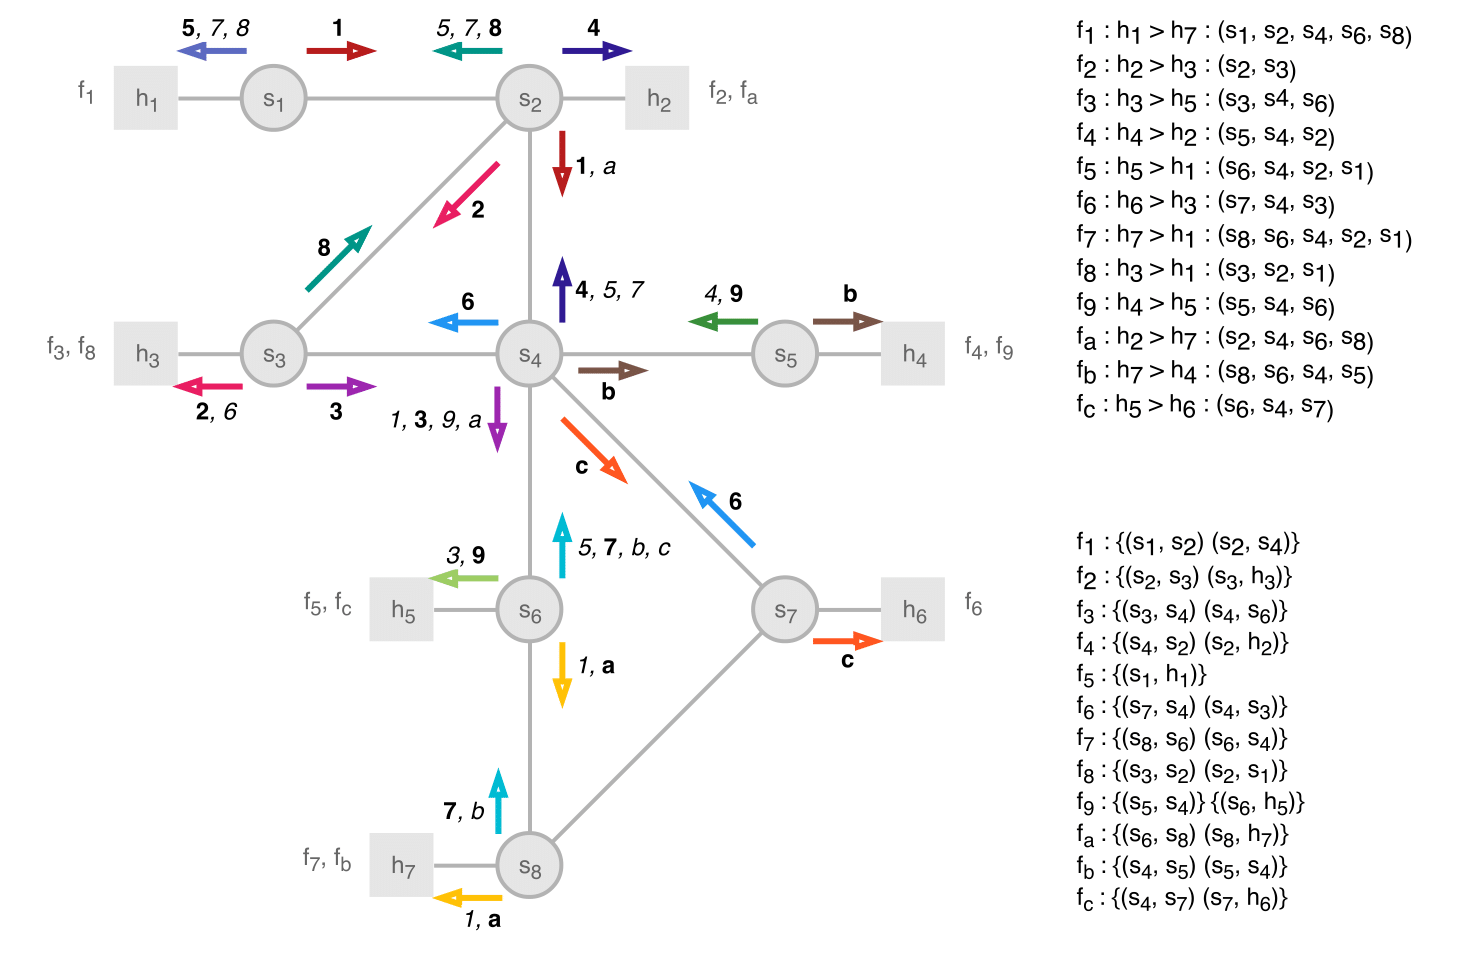
\includegraphics[scale=0.3]{example-topology.png}

To explain how our output would look like in this solution: \\

Note: We are only showing the values which are 1, as to not overcrowd the output. \\

\subsection{Variable X}

\begin{align*}
X[(s1,s2),1] = 1 \\
X[(s2,s4),1] = 1 \\
X[(s2,s3),2] = 1 \\
X[(s3,h3),2] = 1 \\
X[(s3,s4),3] = 1 \\
X[(s4,s6),3] = 1 \\
X[(s4,s2),4] = 1 \\
X[(s2,h2),4] = 1 \\
X[(s1,h1),5] = 1 \\
X[(s7,s4),6] = 1 \\
X[(s4,s3),6] = 1 \\
X[(s8,s6),7] = 1 \\
X[(s6,s4),7] = 1 \\
X[(s3,s2),8] = 1 \\
X[(s2,s1),8] = 1 \\
X[(s5,s4),9] = 1 \\
X[(s6,h5),9] = 1 \\
X[(s6,s8),a] = 1 \\
X[(s8,h7),a] = 1 \\
X[(s6,s6),b] = 1 \\
X[(s5,s4),b] = 1 \\
X[(s4,s7),c] = 1 \\
X[(s7,h6),c] = 1 \\
\end{align*}

\subsection{Variable Y}

\begin{align*}
Y[1,s2] = 1 \\
Y[2,s3] = 1 \\
Y[3,s6] = 1 \\
Y[4,s2] = 1 \\
Y[5,s1] = 1 \\
Y[6,s4] = 1 \\
Y[7,s6] = 1 \\
Y[8,s2] = 1 \\
Y[9,s5] = 1 \\
Y[9,s6] = 1 \\
Y[a,s8] = 1 \\
Y[b,s5] = 1 \\
Y[c,s7] = 1 \\
\end{align*}


\subsection{Variable C}

Note: Since all groups have max size of 2, the weight can is maxed at 1, but if the groups were larger (because of a higher Q capacity), the values could increase. \\

\begin{align*}
C[1,s2] = 1 \\
C[2,s3] = 1 \\
C[3,s4] = 1 \\
C[4,s2] = 1 \\
C[6,s4] = 1 \\
C[7,s6] = 1 \\
C[8,s2] = 1 \\
C[a,s8] = 1 \\
C[b,s5] = 1 \\
C[c,s7] = 1 \\
\end{align*}

\subsection{Objective value}

As we can count the number of 1's in array Y, we find that the objective value found is \textbf{13}. 